\documentclass[aspectratio=169,11pt]{beamer}

\usetheme{default}
\usecolortheme{default}
\setbeamertemplate{navigation symbols}{}
\setbeamertemplate{footline}[frame number]
\setbeamerfont{frametitle}{size=\large,series=\bfseries}
\setbeamercolor{frametitle}{fg=black}
\setbeamertemplate{itemize items}[circle]
\setbeamercolor{itemize item}{fg=black!70}
\setbeamercolor{structure}{fg=black!75}
\setbeamersize{text margin left=7mm, text margin right=7mm}

% Telugu script needs a Unicode engine. Compile with lualatex; the pdflatex
% branch still builds, but renders Telugu examples as blanks.
\usepackage{iftex}
\ifLuaTeX
  \usepackage{fontspec}
  \setmainfont{Latin Modern Roman}
  \setsansfont{Latin Modern Sans}
  \newfontfamily\telugufont[Path=fonts/,
    UprightFont=NotoSansTelugu-Regular.ttf,
    BoldFont=NotoSansTelugu-Bold.ttf, Scale=0.92]{NotoSansTelugu}
\else
  \usepackage[T1]{fontenc}
  \usepackage{lmodern}
  \newcommand{\telugufont}{}
\fi

\usepackage{graphicx}
\usepackage{amsmath,amssymb}
\usepackage{booktabs}
\usepackage{tikz}
\usetikzlibrary{arrows.meta,positioning}

\graphicspath{{images/}}

% Small grey source line for figure attributions.
\newcommand{\src}[1]{{\scriptsize\color{black!55} #1}}
% Slightly tighter item spacing inside frames.
\newcommand{\tight}{\setlength{\itemsep}{2pt plus 1pt minus 1pt}}
% Boxed lead-in or hand-off line, for the narrative bridges.
\newcommand{\bridge}[1]{%
  \vspace{1mm}
  \begin{beamercolorbox}[wd=\textwidth,sep=2mm,rounded=true]{block body}%
    \color{black!80}\small #1
  \end{beamercolorbox}}
% Telugu script inline.
\newcommand{\tel}[1]{{\telugufont #1}}
% Condition labels, so the four conditions always look the same.
\newcommand{\cond}[1]{\textsc{#1}}

\title[Where Does Code-Mixing Break the Task?]{Where Does Code-Mixing Break the Task?\\Function Vectors in Telugu, Romanized Telugu and Tenglish}
\author[2024114003, 2025701032]{Nikhita Ravi (2024114003) \and Krishna Kartheek (2025701032)}
\date{CL3.412 Mechanistic Interpretability of LLMs {\textperiodcentered} Final Project}

\begin{document}

% ------------------------------------------------------------------ title --
\begin{frame}[plain]
  \titlepage
\end{frame}

% ------------------------------------------------------------------ index --
\begin{frame}{Outline}
  \vspace{2mm}
  \begin{columns}[T]
    \begin{column}{0.48\textwidth}
      \begin{enumerate}\small\tight
        \item Problem statement
        \item Background: function vectors
        \item The four conditions
        \item Dataset design
        \item Methodology: causal mediation
        \item Methodology: building the vector
      \end{enumerate}
    \end{column}
    \begin{column}{0.48\textwidth}
      \begin{enumerate}\small\tight
        \setcounter{enumi}{6}
        \item The scaling problem in Gemma 3
        \item Protocol and controls
        \item Results and interpretation
        \item Limitations and negative results
        \item Changes from the proposal, challenges
      \end{enumerate}
    \end{column}
  \end{columns}
\end{frame}

% ----------------------------------------------------------- 1 motivation --
\begin{frame}{Problem statement}
  \begin{columns}[T]
    \begin{column}{0.56\textwidth}
      \begin{itemize}\small\tight
        \item \textbf{Motivation:} Multilingual LLMs degrade on code-mixed
              input, which is how a very large number of people actually
              write. \emph{Where} in the computation this degradation happens
              is not known.
        \vspace{1mm}
        \item \textbf{Research question:} When a model fails on code-mixed
              input, has it lost the \textbf{task representation}, or only the
              ability to \textbf{read the input}?
        \vspace{1mm}
        \item These are different failures with different fixes, and accuracy
              alone cannot tell them apart.
        \vspace{1mm}
        \item \textbf{Our handle:} \textbf{function vectors}, which let us
              extract a task representation and inject it back. If the task
              representation survives, injecting it should repair the failure.
      \end{itemize}
    \end{column}
    \begin{column}{0.44\textwidth}
      \centering
      \vspace{3mm}
      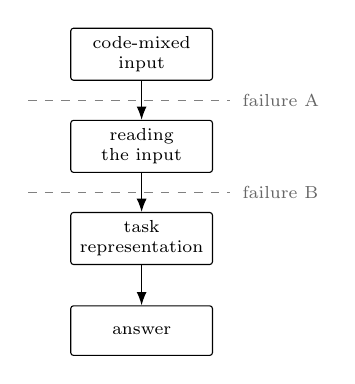
\begin{tikzpicture}[font=\scriptsize, >=Latex, scale=0.9, transform shape,
          b/.style={draw, rounded corners=1pt, minimum width=20mm,
                    minimum height=7mm, align=center}]
        \node[b] (in) at (0,2.6) {code-mixed\\input};
        \node[b] (rd) at (0,1.3) {reading\\the input};
        \node[b] (tk) at (0,0) {task\\representation};
        \node[b] (out) at (0,-1.3) {answer};
        \draw[->] (in) -- (rd);
        \draw[->] (rd) -- (tk);
        \draw[->] (tk) -- (out);
        \node[anchor=west, color=black!60] at (1.3,1.95) {failure A};
        \node[anchor=west, color=black!60] at (1.3,0.65) {failure B};
        \draw[dashed, color=black!50] (-1.6,1.95) -- (1.25,1.95);
        \draw[dashed, color=black!50] (-1.6,0.65) -- (1.25,0.65);
      \end{tikzpicture}\\[1mm]
      \src{Two failure modes a single accuracy number cannot separate.}
    \end{column}
  \end{columns}
\end{frame}

% ------------------------------------------------------- 2 background ------
\begin{frame}{Background: function vectors}
  \begin{columns}[T]
    \begin{column}{0.56\textwidth}
      \begin{itemize}\small\tight
        \item Todd et al. (ICLR 2024) show that in-context learning leaves a
              compact, \textbf{causal} trace of the task in the residual
              stream.
        \item A small set of attention heads carries it. Averaging their
              outputs over many prompts of one task gives a single vector.
        \item Adding that vector to a \textbf{zero-shot} prompt makes the model
              perform the task with no demonstrations at all.
        \item That is the property we need: it is a \emph{measurement} of
              whether the task representation exists, independent of whether
              the prompt is readable.
      \end{itemize}
      \vspace{1mm}
      \begin{itemize}\footnotesize\tight
        \item \textbf{Related work:} causal mediation / activation patching
              (Vig et al., Meng et al.); task vectors (Hendel et al.);
              multilingual interpretability work largely studies clean
              single-language input, not code-mixing.
      \end{itemize}
    \end{column}
    \begin{column}{0.44\textwidth}
      \centering
      \vspace{1mm}
      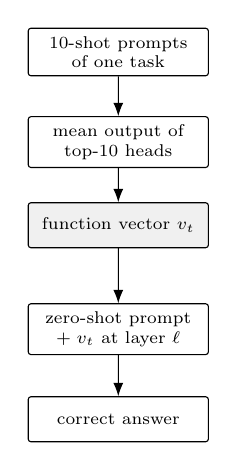
\begin{tikzpicture}[font=\scriptsize, >=Latex, scale=0.88, transform shape,
          b/.style={draw, rounded corners=1pt, minimum width=26mm,
                    minimum height=6.5mm, align=center}]
        \node[b] (p) at (0,3.0) {10-shot prompts\\of one task};
        \node[b] (h) at (0,1.7) {mean output of\\top-10 heads};
        \node[b, fill=black!6] (v) at (0,0.5) {function vector $v_t$};
        \node[b] (z) at (0,-1.0) {zero-shot prompt\\$+\;v_t$ at layer $\ell$};
        \node[b] (a) at (0,-2.3) {correct answer};
        \draw[->] (p) -- (h);
        \draw[->] (h) -- (v);
        \draw[->] (v) -- (z);
        \draw[->] (z) -- (a);
      \end{tikzpicture}
    \end{column}
  \end{columns}
\end{frame}

% -------------------------------------------------- 3 the four conditions --
\begin{frame}{The four conditions}
  Every item exists in four parallel versions. One row of the dataset
  (\texttt{sen-0001}):
  \vspace{2mm}

  {\small
  \begin{tabular}{@{}p{22mm}p{95mm}@{}}
    \toprule
    \cond{en} & next week kavita is buying upma in guntur \\
    \cond{te} & \tel{వచ్చే వారం కవిత గుంటూరులో ఉప్మా కొంటోంది} \\
    \cond{rom} & vachche varam kavita guntur lo upma kontondi \\
    \cond{tg} & \textbf{next week} kavita guntur lo upma kontondi \\
    \bottomrule
  \end{tabular}}

  \vspace{2mm}
  \begin{itemize}\small\tight
    \item \cond{te} is Telugu in its own script; \cond{rom} is the same Telugu
          written in Latin script; \cond{tg} is Tenglish, built \textbf{on top
          of \cond{rom}} by swapping some slots back to English.
    \item That construction is deliberate: \cond{rom} and \cond{tg} share a
          script, so \cond{rom}$\to$\cond{tg} isolates \textbf{code-mixing},
          and \cond{te}$\to$\cond{rom} isolates \textbf{script}.
  \end{itemize}
  \bridge{Conditions are \textbf{row-aligned by item id}, so every comparison is
    paired. The same sentence is tested four ways, which is far more
    statistical power than four independent samples.}
\end{frame}

% ------------------------------------------------------- 4 dataset design --
\begin{frame}{Dataset design}
  \begin{columns}[T]
    \begin{column}{0.52\textwidth}
      \textbf{Two families of tasks}
      \begin{itemize}\footnotesize\tight
        \item \textbf{Part 1 -- word level} (after Todd et al., so our setup is
              comparable to theirs): antonym, present$\to$past,
              singular$\to$plural, next item, and four category/extraction
              tasks. A single word cannot be code-mixed, so these have three
              conditions.
        \item \textbf{Part 2 -- sentence level} (ours): from a sentence, extract
              the \textbf{person}, \textbf{place}, \textbf{food} or
              \textbf{verb}; or label its \textbf{tense},
              \textbf{polarity} or \textbf{subject gender}. All four
              conditions.
      \end{itemize}
      \vspace{1mm}
      \textbf{Tiers, to test degradation on purpose}
      \begin{itemize}\footnotesize\tight
        \item \texttt{core}, \texttt{complex}, \texttt{sanskritized},
              \texttt{rare}, \texttt{literary\_en}, \texttt{ambiguous}.
        \item Headline numbers use \texttt{core} only; the harder tiers are
              held back so difficulty never silently drives a result.
      \end{itemize}
    \end{column}
    \begin{column}{0.48\textwidth}
      \centering
      \src{Items per task and tier (abridged)}\\[1mm]
      {\scriptsize\setlength{\tabcolsep}{3.0pt}
      \begin{tabular}{lrrrr}
        \toprule
        task & core & cplx & skrt & total \\
        \midrule
        antonym          & 127 & 10 & 15 & 167 \\
        present past     & 108 & 20 & 16 & 159 \\
        singular plural  & 122 & 30 & 15 & 180 \\
        next item        &  67 & 26 & 15 & 123 \\
        extract person   & 200 & 50 & 0 & 250 \\
        extract place    & 298 & 102 & 0 & 400 \\
        extract food     & 298 & 102 & 0 & 400 \\
        extract verb     & 298 & 102 & 0 & 400 \\
        negation         & 148 & 50 & 0 & 198 \\
        subject gender   &  48 & 26 & 0 &  74 \\
        \bottomrule
      \end{tabular}}
      \\[1.5mm]
      \src{Hand-written TSV, no code in \texttt{data/}, extensible by adding
        rows: splits are content-addressed so they do not move.}
    \end{column}
  \end{columns}
\end{frame}

% ------------------------------------------- 5 what romanization costs -----
\begin{frame}{What the conditions actually cost the model}
  \begin{columns}[T]
    \begin{column}{0.5\textwidth}
      \textbf{Romanization is lossy and inconsistent}
      \begin{itemize}\footnotesize\tight
        \item Telugu distinguishes length and aspiration that Latin script,
              as people actually type it, does not: \tel{వేడి} /
              \tel{చల్లని} become \texttt{vedi} / \texttt{challani}.
        \item Morphology survives as an opaque string:
              \tel{గుర్తుంచుకోవడం} $\to$ \texttt{gurtunchukovadam}, a
              multi-suffix verbal noun with no visible boundaries.
        \item We fix one convention and document its losses, rather than
              pretend it is reversible.
      \end{itemize}
    \end{column}
    \begin{column}{0.5\textwidth}
      \textbf{Why subject gender is the sharp test}
      \vspace{1mm}
      {\footnotesize
      \begin{tabular}{@{}llp{18mm}@{}}
        \toprule
        gender & Telugu & English \\
        \midrule
        masc. & \tel{తిన్నాడు} \,(\texttt{tinnadu}) & ate \\
        fem.  & \tel{తింది} \,(\texttt{tindi}) & ate \\
        \bottomrule
      \end{tabular}}
      \vspace{1.5mm}
      \begin{itemize}\footnotesize\tight
        \item The Telugu verb marks the subject's gender; the English verb does
              not. Same meaning, different information content.
        \item So \cond{en} \textbf{cannot} be above chance on this task, by
              construction. It is our built-in sanity check: a method that
              reports success on \cond{en} here is measuring an artefact.
      \end{itemize}
    \end{column}
  \end{columns}
\end{frame}

% ------------------------------------------- 6 methodology: mediation ------
\begin{frame}{Methodology: finding the heads by causal mediation}
  \begin{itemize}\small\tight
    \item For each attention head, we measure its \textbf{indirect effect}:
          how much of the task behaviour it is responsible for.
  \end{itemize}
  \vspace{1mm}
  \centering
  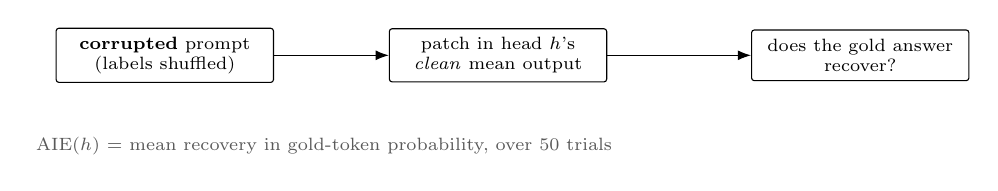
\begin{tikzpicture}[font=\scriptsize, >=Latex, scale=0.92, transform shape,
      b/.style={draw, rounded corners=1pt, minimum width=30mm,
                minimum height=7mm, align=center}]
    \node[b] (c) at (0,0) {\textbf{corrupted} prompt\\(labels shuffled)};
    \node[b] (p) at (4.6,0) {patch in head $h$'s\\\emph{clean} mean output};
    \node[b] (m) at (9.6,0) {does the gold answer\\recover?};
    \draw[->] (c) -- (p);
    \draw[->] (p) -- (m);
    \node[anchor=west, font=\scriptsize, color=black!65] at (-1.9,-1.25)
      {AIE$(h)$ = mean recovery in gold-token probability, over 50 trials};
  \end{tikzpicture}
  \vspace{2mm}
  \begin{itemize}\small\tight
    \item Rank heads by AIE, keep the \textbf{top 10} (as in Todd et al.).
    \item \textbf{Our deviation:} we compute a head set \textbf{per condition},
          not one universal set. That is the whole point --- we want to know
          whether \cond{te}, \cond{rom} and \cond{tg} recruit the same
          mechanism as \cond{en}, and a shared set would assume the answer.
    \item \textbf{Cost control:} all heads of a layer are patched in one
          batched forward, so a trial costs $n_{\text{layers}}$ forwards
          instead of $n_{\text{layers}}\times n_{\text{heads}}$. Without this
          the sweep is ${\sim}50$ hours instead of ${\sim}1.5$.
  \end{itemize}
\end{frame}

% --------------------------------------- 7 methodology: building the vector
\begin{frame}{Methodology: building and injecting the vector}
  \begin{columns}[T]
    \begin{column}{0.54\textwidth}
      \begin{itemize}\footnotesize\tight
        \item For each task $t$ and condition $c$, average each selected head's
              output over 100 ten-shot prompts, giving $\bar a_h$.
        \item Sum those through the output projection:
      \end{itemize}
      \vspace{-1mm}
      \begin{equation*}\small
        v_{t,c} \;=\; \sum_{h \in \mathcal{H}_c} W_O^{(h)}\, \bar a_h
      \end{equation*}
      \begin{itemize}\footnotesize\tight
        \item Then add $v_{t,c}$ to the residual stream at \textbf{one} layer
              $\ell$ of a \textbf{zero-shot} prompt and read the next token.
        \item \textbf{Scoring:} first-token exact match against the gold
              answer. Every answer in the dataset was linted to be
              single-token-decidable.
        \item \textbf{Competence filter:} an item counts only if the model
              already gets it right at 10 shots (gold-token rank 0). We are
              asking whether the \emph{vector} works, not whether the model
              knows the word.
      \end{itemize}
    \end{column}
    \begin{column}{0.46\textwidth}
      \centering
      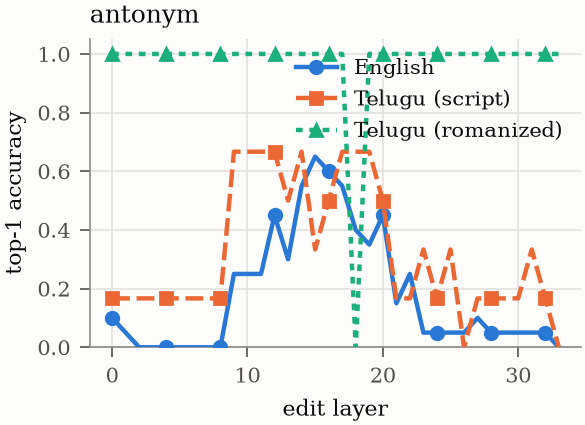
\includegraphics[width=\linewidth]{layer_sweep.png}\\[1mm]
      \src{Zero-shot accuracy with the vector injected at each layer. The
        effect is mid-depth, as reported for GPT-J.}
    \end{column}
  \end{columns}
\end{frame}

% ------------------------------------- 8 the scaling problem (key slide) ---
\begin{frame}{The scaling problem in Gemma 3}
  \bridge{Our first full run showed the function vector changing
    \textbf{nothing}: $+0.00$ at every layer, in every condition, including
    English. The method had not failed --- the arithmetic had.}
  \begin{columns}[T]
    \begin{column}{0.52\textwidth}
      \begin{itemize}\footnotesize\tight
        \item Gemma scales embeddings by $\sqrt{d_{\text{model}}}$ and never
              renormalises the stream, so $\|h_\ell\|$ grows from ${\sim}780$
              at layer 0 to ${\sim}10^5$ at layer 33.
        \item A function vector has norm ${\sim}16$--$22$. Adding it raw is a
              \textbf{0.1\% nudge}: real, but far too small to move an argmax
              over a 262k vocabulary.
        \item GPT-J, which the method was built on, does not have this gap --- so
              nothing in the original work flags it.
        \item \textbf{Fix:} scale the vector to a fraction $\alpha$ of the
              residual norm at the edit layer,
              $v \leftarrow v \cdot \alpha\|h_\ell\| / \|v\|$, with $\alpha$
              chosen on a dev slice.
      \end{itemize}
    \end{column}
    \begin{column}{0.48\textwidth}
      \centering
      \src{Effect of the fix, held-out accuracy}\\[1mm]
      {\footnotesize\setlength{\tabcolsep}{4pt}
      \begin{tabular}{llcc}
        \toprule
        task & cond. & raw & scaled \\
        \midrule
        extract verb   & \cond{en} & 0.00 & \textbf{0.99} \\
        extract place  & \cond{en} & 0.00 & \textbf{0.98} \\
        subject gender & \cond{te} & 0.00 & \textbf{0.89} \\
        present past   & \cond{te} & 0.00 & \textbf{1.00} \\
        \bottomrule
      \end{tabular}}
      \\[2mm]
      \begin{itemize}\footnotesize\tight
        \item Selected multipliers run from $35\times$ to $1841\times$.
        \item \textbf{This is a transferable finding:} function vectors do not
              port to Gemma-class models until they are rescaled relative to
              the residual norm.
      \end{itemize}
    \end{column}
  \end{columns}
\end{frame}

% ------------------------------------------- 9 protocol and controls -------
\begin{frame}{Protocol and controls}
  \begin{columns}[T]
    \begin{column}{0.5\textwidth}
      \textbf{Keeping ourselves honest}
      \begin{itemize}\footnotesize\tight
        \item Both free parameters --- the edit layer $\ell$ and the scale
              $\alpha$ --- are chosen on a \textbf{30\% dev slice} and reported
              on the held-out remainder.
        \item Layer selection uses a smoothed curve with a mid-depth
              tie-break. A plain argmax silently resolved all-zero ties to
              layer 0.
        \item Splits are content-addressed hashes, so adding dataset rows
              does not reshuffle existing splits.
        \item Every number is stamped with a config hash covering configs
              \emph{and} code version, so a stale cache cannot be replayed as
              a result.
      \end{itemize}
    \end{column}
    \begin{column}{0.5\textwidth}
      \textbf{Four controls, each closing one story}
      \begin{itemize}\footnotesize\tight
        \item \textbf{Random vector, matched norm} --- rules out ``any large
              vector at that depth jolts the model''.
        \item \textbf{Unrelated-task function vector} --- rules out ``any
              well-formed function vector helps''.
        \item \textbf{Shuffled-label floor} --- the level reached when the
              prompt has the task's form but not its content.
        \item \textbf{Majority-class floor} --- on 2- and 3-way label tasks, an
              accuracy without its floor is not interpretable.
      \end{itemize}
      \vspace{1mm}
      \src{All three injected vectors are scaled to the \emph{same} norm, so
        the only thing that differs is direction.}
    \end{column}
  \end{columns}
\end{frame}

% --------------------------------------------------- 10 results: baselines -
\begin{frame}{Results: the degradation is real, and task-dependent}
  \begin{columns}[T]
    \begin{column}{0.46\textwidth}
      \centering
      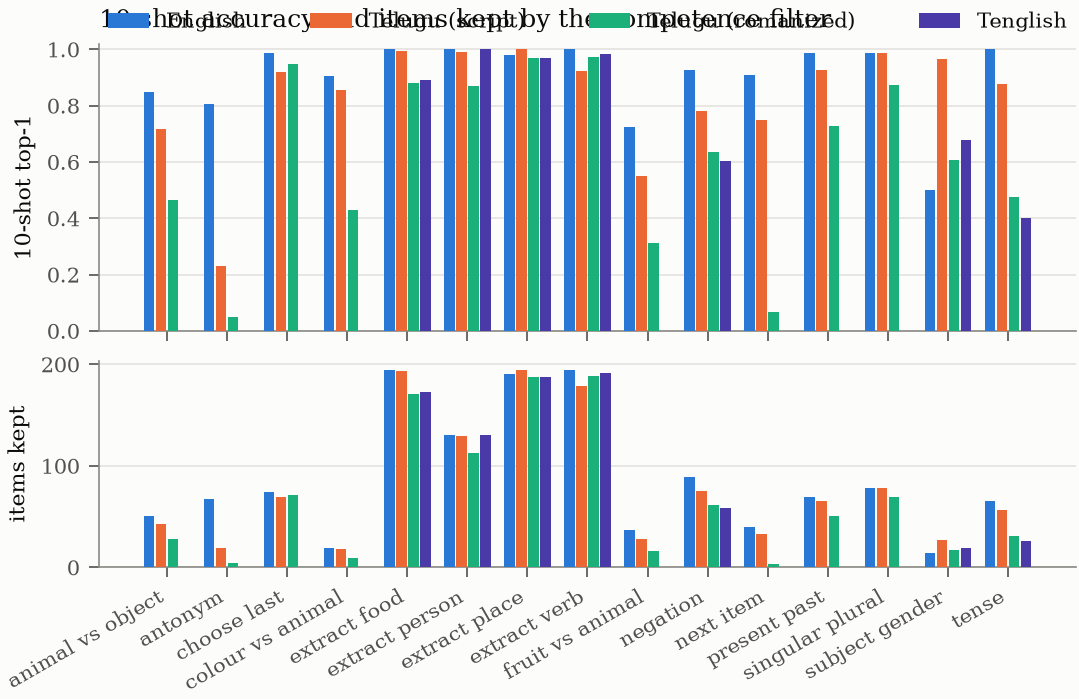
\includegraphics[width=\linewidth]{baselines.png}\\[1mm]
      \src{10-shot accuracy, Gemma 3 4B, \texttt{core} tier.}
    \end{column}
    \begin{column}{0.54\textwidth}
      \begin{itemize}\small\tight
        \item \textbf{Copy-style tasks sit at ceiling everywhere.} Extracting a
              place or a person is ${\ge}0.97$ in all four conditions ---
              romanization does not hurt at all.
        \item \textbf{Reasoning-style tasks degrade monotonically}
              \cond{en}$\to$\cond{te}$\to$\cond{rom}$\to$\cond{tg}:
              negation $0.93 \to 0.78 \to 0.64 \to 0.60$.
        \item \textbf{Subject gender inverts}, exactly as the linguistics
              predicts: \cond{en} $0.50$ (chance, no gender marking available)
              against \cond{te} $0.96$.
        \item \textbf{Romanized word-level tasks lose most of their items} to
              the competence filter: antonym keeps 4 of 167. Those cells are
              reported but carry no weight.
      \end{itemize}
    \end{column}
  \end{columns}
\end{frame}

% ------------------------------------------------- 11 results: head sets ---
\begin{frame}{Results: the same heads, in every condition}
  \begin{columns}[T]
    \begin{column}{0.44\textwidth}
      \centering
      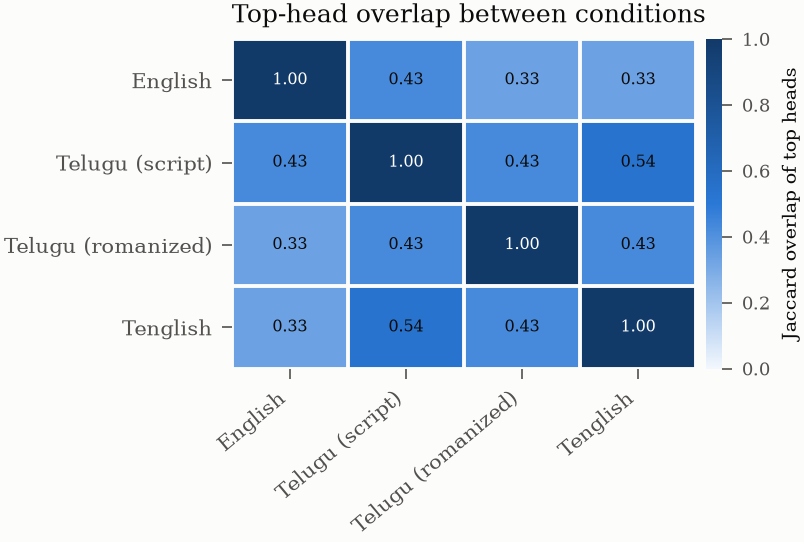
\includegraphics[width=\linewidth]{head_overlap.png}\\[1mm]
      \src{Jaccard overlap of the top-10 head sets.}
    \end{column}
    \begin{column}{0.56\textwidth}
      {\scriptsize\setlength{\tabcolsep}{3pt}
      \begin{tabular}{ll}
        \toprule
        condition & top heads (layer.head) \\
        \midrule
        \cond{en}  & \texttt{17.4, 17.6, 13.2, 22.3, 17.5, 18.7, \ldots} \\
        \cond{te}  & \texttt{17.4, 17.6, 17.5, 13.2, 22.3, 18.1, \ldots} \\
        \cond{rom} & \texttt{17.6, 17.4, 22.3, 17.5, 13.2, 21.7, \ldots} \\
        \cond{tg}  & \texttt{17.4, 17.6, 22.3, 17.5, 18.1, 23.1, \ldots} \\
        \bottomrule
      \end{tabular}}
      \vspace{2mm}
      \begin{itemize}\small\tight
        \item \textbf{Heads 17.4 and 17.6 are top-2 in all four conditions},
              at layer 17 of 34 --- mid-depth, replicating the depth finding
              from GPT-J in a different architecture and a different language.
        \item Overlap: \cond{en}--\cond{te} $0.43$,
              \cond{en}--\cond{rom} $0.33$, \cond{en}--\cond{tg} $0.33$,
              \cond{te}--\cond{tg} $\mathbf{0.54}$.
        \item \textbf{English is the outlier}, not Tenglish. The three
              Telugu-derived conditions resemble each other more than any
              resembles English.
      \end{itemize}
    \end{column}
  \end{columns}
  \bridge{So code-mixing does \textbf{not} recruit a separate mechanism. Whatever
    breaks, it is not that the model routes Tenglish somewhere else.}
\end{frame}

% ------------------------------------------------ 12 results: FV efficacy --
\begin{frame}{Results: does the injected vector repair the failure?}
  \centering
  \src{Held-out accuracy of a zero-shot prompt plus the function vector,
    Gemma 3 4B. 95\% bootstrap CIs in the report.}\\[1.5mm]
  {\small\setlength{\tabcolsep}{5pt}
  \begin{tabular}{lcccc}
    \toprule
    task & \cond{en} & \cond{te} & \cond{rom} & \cond{tg} \\
    \midrule
    extract place   & 0.98 & 0.99 & 0.76 & 0.83 \\
    extract person  & 0.84 & 0.96 & 0.85 & 0.93 \\
    \midrule
    extract verb    & 0.99 & 0.93 & \textbf{0.21} & \textbf{0.30} \\
    extract food    & 0.80 & 0.81 & \textbf{0.33} & \textbf{0.39} \\
    \midrule
    subject gender  & 0.80 & 0.89 & \textbf{0.00} & \textbf{0.00} \\
    present past    & 0.29 & 1.00 & 0.81 & -- \\
    tense           & 0.00 & 0.00 & 0.00 & 0.00 \\
    \bottomrule
  \end{tabular}}
  \vspace{2mm}
  \begin{itemize}\small\tight
    \item \textbf{Telugu script recovers; Latin script does not.} For
          \texttt{extract\_verb} the vector takes \cond{te} to $0.93$ but
          \cond{rom} only to $0.21$ --- from the \emph{same} sentences, differing
          only in script.
    \item But the collapse is \textbf{not uniform}: person and place extraction
          survive romanization fine. Only some tasks fall off the cliff.
  \end{itemize}
\end{frame}

% ------------------------------------------ 13 results: majority floors ----
\begin{frame}{Results: reading the label tasks honestly}
  \begin{columns}[T]
    \begin{column}{0.52\textwidth}
      {\footnotesize\setlength{\tabcolsep}{4pt}
      \begin{tabular}{llrrr}
        \toprule
        task & cond. & $n$ & major. & +FV \\
        \midrule
        negation & \cond{en} & 62 & 0.53 & 0.53 \\
        negation & \cond{rom} & 43 & 0.77 & 0.77 \\
        negation & \cond{tg} & 41 & 0.80 & 0.39 \\
        \midrule
        subj. gender & \cond{en} & 10 & 0.90 & 0.80 \\
        subj. gender & \cond{te} & 19 & 0.58 & \textbf{0.89} \\
        subj. gender & \cond{rom} & 12 & 0.75 & 0.00 \\
        \midrule
        tense & \cond{en} & 45 & 0.44 & 0.00 \\
        \bottomrule
      \end{tabular}}
    \end{column}
    \begin{column}{0.48\textwidth}
      \begin{itemize}\footnotesize\tight
        \item An accuracy equal to the majority rate is the signature of a
              model emitting \textbf{one label for everything}. Negation
              \cond{en} and \cond{rom} match their floors exactly.
        \item \textbf{Of twelve label-task cells, exactly one clears its
              floor:} subject gender in \cond{te}, $0.89$ against $0.58$.
        \item That one is the cell where the linguistics says the information
              is actually present --- and \cond{en} at $0.80$ sits
              \emph{below} its $0.90$ floor, which is the sanity check firing
              correctly.
        \item \textbf{We therefore report the other label cells as ``not above
              chance'', not as accuracies.}
      \end{itemize}
    \end{column}
  \end{columns}
  \bridge{Without the floor beside it, \cond{en} subject gender at $0.80$ would
    have read as a strong positive result. It is the opposite.}
\end{frame}

% ---------------------------------------------------- 14 interpretation ----
\begin{frame}{Interpretation: what breaks is reading, not the task}
  \begin{itemize}\small\tight
    \item \textbf{The task representation survives code-mixing.} The same
          mid-layer heads carry it in all four conditions (overlap peaks
          between \cond{te} and \cond{tg}, not within English), and a vector
          extracted under code-mixing is built from the same mechanism.
    \vspace{1mm}
    \item \textbf{What fails is recovering the argument from the surface
          form.} The dissociation in our own results makes this concrete:
  \end{itemize}
  \vspace{1mm}
  \begin{columns}[T]
    \begin{column}{0.48\textwidth}
      \textbf{Survives romanization}
      \begin{itemize}\footnotesize\tight
        \item \texttt{extract\_person} $0.85$ / $0.93$
        \item \texttt{extract\_place} \; $0.76$ / $0.83$
        \item These targets are \textbf{proper nouns}. ``kavita'', ``guntur''
              romanize essentially losslessly --- the string is the same object.
      \end{itemize}
    \end{column}
    \begin{column}{0.48\textwidth}
      \textbf{Collapses under romanization}
      \begin{itemize}\footnotesize\tight
        \item \texttt{extract\_verb} \; $0.21$ / $0.30$
        \item \texttt{subject\_gender} $0.00$ / $0.00$
        \item These targets live in \textbf{inflectional morphology}.
              \tel{కొంటోంది} $\to$ \texttt{kontondi} is where tense, gender and
              polarity are encoded, and romanization flattens it.
      \end{itemize}
    \end{column}
  \end{columns}
  \bridge{\textbf{Answer to the research question:} code-mixing breaks the task at
    the \emph{input-reading} stage, and selectively --- it damages what is
    carried by morphology while leaving what is carried by identifiable
    substrings intact.}
\end{frame}

% ----------------------------------- 15 limitations and negative results ---
\begin{frame}{Limitations and negative results}
  \begin{columns}[T]
    \begin{column}{0.5\textwidth}
      \textbf{Negative results we are reporting}
      \begin{itemize}\footnotesize\tight
        \item \textbf{\texttt{tense} fails everywhere, English included}
              ($0.00$ at every layer and every scale). A condition effect
              would show as a gap; a flat zero in the control language is a
              \textbf{method limitation on that task}, so we report it as one
              rather than quietly dropping it.
        \item \textbf{Transfer and the vector-specificity controls are being
              recomputed.} We found that both stages were applying the vector
              at its \emph{raw} norm --- the same bug the scaling fix solved
              elsewhere --- which made every control equal the function vector.
              Those cells are not reported until the rerun lands.
      \end{itemize}
    \end{column}
    \begin{column}{0.5\textwidth}
      \textbf{Scope}
      \begin{itemize}\footnotesize\tight
        \item \textbf{One model family} (Gemma 3), one size reported here.
              The scaling finding is specifically about Gemma-class residual
              growth.
        \item \textbf{Small cells.} Romanized word-level tasks keep 2--13 items
              after the competence filter. We show them, but draw no
              conclusions from them.
        \item \textbf{Word order is a confound} for \cond{en}--\cond{te}
              similarity: English is SVO and Telugu SOV, so the vectors differ
              for a reason unrelated to script. \cond{rom}--\cond{tg} is the
              clean comparison.
        \item \textbf{One romanization convention}, chosen and documented.
              Real users are inconsistent in ways we do not model.
      \end{itemize}
    \end{column}
  \end{columns}
\end{frame}

% --------------------------------------------- 16 changes from proposal ----
\begin{frame}{What changed from the proposal}
  \begin{columns}[T]
    \begin{column}{0.5\textwidth}
      \textbf{Dropped}
      \begin{itemize}\footnotesize\tight
        \item \textbf{Incremental $\pm$ scoring} of newly added dataset rows.
              Refitting from scratch is cheap enough with caching, and
              incremental scoring would have made every number depend on
              insertion order.
        \item \textbf{vLLM for the Gemma runs.} vLLM cannot expose or patch
              intermediate activations, which is the entire experiment. Plain
              \texttt{transformers} with hooks it is.
        \item \textbf{The \texttt{tense} task as a headline result} --- kept in
              the tables, reported as a method limitation.
      \end{itemize}
    \end{column}
    \begin{column}{0.5\textwidth}
      \textbf{Changed or added}
      \begin{itemize}\footnotesize\tight
        \item \textbf{27B $\to$ 12B} as the second model, on compute cost.
        \item \textbf{Per-condition head sets} instead of one universal set ---
              without this we could not have measured head overlap, which
              turned out to be a main result.
        \item \textbf{Residual-relative scaling}, which was not in the plan
              because we did not know it was needed. It is now arguably the
              most portable contribution.
        \item \textbf{Majority-class floors}, added after noticing that
              \cond{en} subject gender looked like a success.
      \end{itemize}
    \end{column}
  \end{columns}
\end{frame}

% --------------------------------------------------- 17 challenges ---------
\begin{frame}{Challenges faced}
  \begin{columns}[T]
    \begin{column}{0.5\textwidth}
      \textbf{Infrastructure}
      \begin{itemize}\footnotesize\tight
        \item The cluster's documentation did not match the cluster: wrong
              partition name, modules that do not exist on its actual OS,
              node names in a different format.
        \item A \texttt{venv} built from inside an active \texttt{venv}
              resolved its own interpreter and produced
              \texttt{No module named torch} only on compute nodes.
        \item \textbf{fp16 produced NaNs} in Gemma 3 mediation on the
              available GPUs, so the whole project moved to a rented H200 in
              bf16.
        \item A concurrent 27B download filled the volume mid-run and killed
              the job; the fetch script now pre-checks free space.
      \end{itemize}
    \end{column}
    \begin{column}{0.5\textwidth}
      \textbf{Scientific debugging}
      \begin{itemize}\footnotesize\tight
        \item \textbf{Three separate bugs all presented as ``the function
              vector does nothing''}: layer selection collapsing to layer 0 on
              ties, a config hash that did not cover code version so stale
              results replayed, and the residual-scale problem.
        \item Only the last was real science. Finding it needed a purpose-built
              diagnostic that printed
              $\|v\|$ against $\|h_\ell\|$ --- the ratio was $0.001$.
        \item \textbf{Lesson we would keep:} make every stage print the
              quantity it depends on. A result of exactly $+0.00$ should be
              treated as a bug report, not a finding.
      \end{itemize}
    \end{column}
  \end{columns}
\end{frame}

% --------------------------------------------------- 18 conclusion --------
\begin{frame}{Conclusion}
  \bridge{\textbf{Code-mixing does not give the model a different task
    representation. It makes the input harder to read --- and specifically, it
    damages what Telugu encodes in morphology while leaving what it encodes in
    identifiable substrings intact.}}
  \vspace{1mm}
  \begin{columns}[T]
    \begin{column}{0.32\textwidth}
      \textbf{What we showed}
      \begin{itemize}\footnotesize\tight
        \item The same mid-layer heads carry the task in all four conditions;
              English is the outlier, not Tenglish.
        \item Injecting the vector repairs Telugu script but not Latin script,
              on the same sentences.
        \item Proper-noun targets survive; morphology-borne targets collapse.
      \end{itemize}
    \end{column}
    \begin{column}{0.32\textwidth}
      \textbf{Methods contribution}
      \begin{itemize}\footnotesize\tight
        \item Function vectors do not transfer to Gemma-class models until
              rescaled relative to the residual norm --- a $35$--$1841\times$
              correction.
        \item A paired, four-condition dataset with explicit difficulty tiers,
              hand-editable and extensible.
      \end{itemize}
    \end{column}
    \begin{column}{0.32\textwidth}
      \textbf{In progress}
      \begin{itemize}\footnotesize\tight
        \item \textbf{Gemma 3 12B} on the subset of tasks where 4B degraded,
              to test whether scale closes the romanization gap.
        \item Recomputed transfer matrix and specificity controls.
        \item Pooling the small romanized word-level cells.
      \end{itemize}
    \end{column}
  \end{columns}
\end{frame}

% --------------------------------------------------------------- thanks ---
\begin{frame}[plain]
  \vfill
  \centering
  {\Large Thank you}\\[6mm]
  {\large Questions?}\\[12mm]
  {\small Todd, Li, Sharma, Mueller, Wallace, Bau.\\
   Function Vectors in Large Language Models. ICLR 2024.\\[2mm]
   Code and dataset: \texttt{github.com/<user>/MechInterp-final-project}}
  \vfill
\end{frame}

\end{document}
